\documentclass{standalone}
\usepackage{tikz}
\usepackage{makecell}

\begin{document}	
	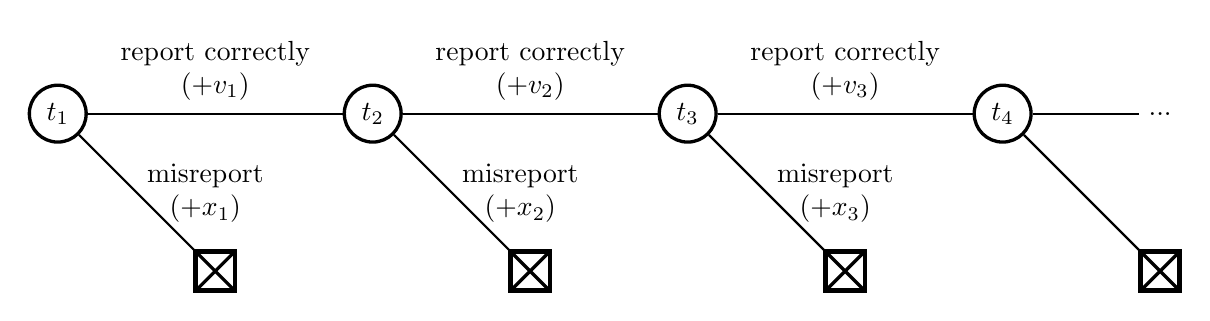
\begin{tikzpicture}[scale=2]
	
	\tikzset{cross/.style={path picture={\draw[black, very thick] (path picture bounding box.south east) -- (path picture bounding box.north west) (path picture bounding box.south west) -- (path picture bounding box.north east);}}}
	
	
	\node[circle, draw, very thick] at (0,0) (t1) {$t_1$};
	\node[circle, draw, very thick] at (2,0) (t2) {$t_2$};
	\node[circle, draw, very thick] at (4,0) (t3) {$t_3$};
	\node[circle, draw, very thick] at (6,0) (t4) {$t_4$};
	\node at (7,0) (t5) {...};
	
	\node[rectangle, draw, fill=black, scale=2.25, thick] at (1,-1) {};
	\node[rectangle, draw, fill=white, scale=2, thick, cross] at (1,-1) (e1) {};
	\node[rectangle, draw, fill=black, scale=2.25, thick] at (3,-1) {};
	\node[rectangle, draw, fill=white, scale=2, thick, cross] at (3,-1) (e2) {};
	\node[rectangle, draw, fill=black, scale=2.25, thick] at (5,-1) {};
	\node[rectangle, draw, fill=white, scale=2, thick, cross] at (5,-1) (e3) {};\\
	\node[rectangle, draw, fill=black, scale=2.25, thick] at (7,-1) {};
	\node[rectangle, draw, fill=white, scale=2, thick, cross] at (7,-1) (e4) {};
	
	\draw[thick] (t1) -- (t2) node[midway, above, align=center] {\makecell[c]{report correctly\\ ($+v_1$)}};
	\draw[thick] (t2) -- (t3) node[midway, above, align=center] {\makecell[c]{report correctly\\ ($+v_2$)}};
	\draw[thick] (t3) -- (t4) node[midway, above, align=center] {\makecell[c]{report correctly\\ ($+v_3$)}};
	\draw[thick] (t4) -- (t5);
	
	\draw[thick] (t1) -- (e1) node[midway, right, align=center] {\makecell[c]{misreport\\ ($+x_1$)}};
	\draw[thick] (t2) -- (e2) node[midway, right, align=center] {\makecell[c]{misreport\\ ($+x_2$)}};
	\draw[thick] (t3) -- (e3) node[midway, right, align=center] {\makecell[c]{misreport\\ ($+x_3$)}};
	\draw[thick] (t4) -- (e4);
	
	
	\end{tikzpicture}
\end{document}